\documentclass[a4papaer.12pt]{article}
\usepackage[top=1.5in, bottom=1.5in, left= 1.5in, right=1.5in]{geometry}
\usepackage{apacite}
\usepackage{enumerate}
\usepackage{graphicx}
\usepackage{array}
\graphicspath{{C:\Users\asus\Desktop\Assignment2}}

\begin{document}
\bibliographystyle{apacite}

\title{\textbf{Using SentiWordNet for Multilingual Sentiment Analysis}}
\author{\textbf{Fam Jiang Yuan}}
\date{}
\maketitle

\section*{\textbf{Executive Summary}}
In this paper, we proposed a Multilingual Sentiment Analysis method to determining the sentiment of texts in other languages. There are tons of information on Internet, some are written in other languages. Meanwhile, a lots of valuable data that written in other language are not collected. Therefore, we introduce a methodology to overcome the problem. Our proposed method is able to determine the sentiment of texts in multilingual framework, which benefits a lots to opinion mining. By achieving our method, we used a translation software to translate the documents that written in different languages into English first and then classified accordingly into "positive" and "negative". Next, SentiWordNet is used calculate the scores for positivity and negativity. Our proposed method is tested in German movie reviews and the outcomes show that our method is achievable for multilingual sentiment analysis.
 
\section*{\textbf{Introduction}}
The information on Internet nowadays have became more important and valuable for other purposes, such as marketing, opinions, reviews, and many more. However, some information are written in different language that other than English. 
\\
\\
In order to collect those data that written in different language, we proposed a methodology that can automatically differentiate the polarity of texts in multiple languages without specific lexicon and without specific training data. The training material is spare, due to the multilingual framework. Therefore, the polarity is measured by using a lexicon-based method in English term.
\\
\\  
Three types of classifier are used on our research to determining the polarity of texts and sentiment classification, which are LingPipe Classifier, SentiWordNet Classifier with classification rule, and SentiWord Classifier with machine learning. Three classifier are tested with same and specific language documents and the outcomes are annotated accordingly. 

\pagebreak
\section*{\textbf{Justification of Research}}
The propose to carry out this research is to fetch up human capability, as such large quantity of texts and opinions,and some are written by different language on Internet everyday. Yet, our research can reduce human effort by determining the sentiment of collected texts automatically.

\section*{\textbf{Research Objectives}}
\begin{itemize}
\item To fetch up human capabilities on handling large quantity of data from multilingual.
\item To reduce human effort on opinion mining by determining the sentiment of texts automatically.
\item To enhance the current existing method for multilingual sentiment analysis and opinion mining.
\end{itemize}

\section*{\textbf{Literature Review}}
\begin{enumerate}[I]
\item \textit{Multilingual Sentiment Analysis}
\\
There are a few difficulties that multilingual sentiment analysis offered, which are the training materials form multilingual is sparse and generating these training resources is taking a lot of time and human effort is needed. 
\\
\\
Referring to the existing research, \cite{mihalcea2007learning} using corpus-based method and lexicon-based method to multilingual subjective text analysis. \cite{almas2007note} is using a local grammar method for multilingual sentiment classification. 
\\
\\Both mentioned methods do not perform the sentiment analysis of the texts. Method of \cite{mihalcea2007learning} is to differentiate subjective texts. \cite{almas2007note} only able to determine the sentiment bearing phrases. Whereas the sentiment of the sentences and polarity are remain undetermined. 
\\
\item \textit{Sentiment Analysis based on SentiWordNet}
\\
In our paper, we are using SentiWordNet as our lexical resource. Each synset of WordNet in SentiWordNet is assigned a score triple. There are a few existing works been done by \cite{devitt2007sentiment} on detecting the sentiment polarity in financial news. \cite{chaumartin2007upar7} used SentiWordNet on headlines. Both approaches are done in monolingual framework.
\end{enumerate}

\pagebreak

\section*{\textbf{Research Methodology}}
\begin{enumerate}[I]
\item \textit{Language Classification}
\\
LingPipe Language Identification Classifier has been trained by text corpora that consists 15 different languages. LingPipe is used to identify the language by using Character-based language models, which assigns probability to texts sequence. An n-gram model with size of eight is used in text classification. Character-based language models are also successfully functioned in other tasks in text classification, such as spam detection in \cite{wilson2005recognizing}. 
\\
\item \textit{Language Standardization}
\\
For collecting opinions and reviews from different languages to English, a language translation software is used. Each document that written in different language is automatically translated into English. In our experiment, we are using PROMT Translation technology to do the translation works.
\\

\begin{center}
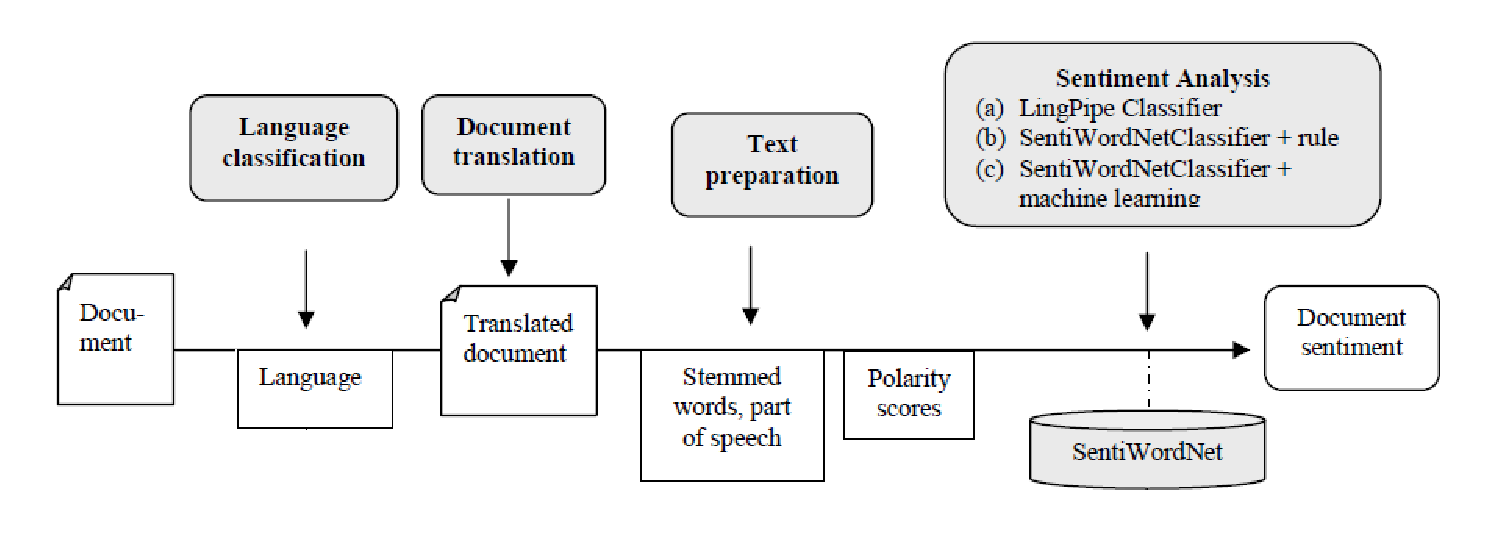
\includegraphics[scale=0.5]{Assignment2}
\\
\textbf{Figure 1}: Processing pipeline for sentiment analysis
\end{center}

\item \textit{Sentiment Classification}
\\
LingPipe classifier is used for determining the polarity of texts and then classified  into positive and negative document. LingPipe classifier is trained by English document, due to the training material is difficult to obtain.
\\
\\
For SentiWordNet Classifier with classification rule, the sentiment polarity is obtained form document polarity. However, the document must be divided into sentences first, and each sentiment score triple (score{\tiny pos}, socre{\tiny neg}, score{\tiny obj})are determined by SentiWordNet.
\\
\\
For SentiWordNet with machine learning, the score triple for each sentences has been provided in WEKA package, \cite{esuli2006sentiwordnet}. Next, each word in the sentence is stemmed and distributed the Part of Speech(POS) tag. The SentiWordNet with machine learning calculated the score triple for each sentences by means of positive, negative, and objective scores.
\end{enumerate}

\pagebreak

\bibliography{mybib2}
\bibliographystyle{plain}

\pagebreak

\begin{center}
\begin{tabular}{|m{5cm} | m{10cm} |}
\hline
Paper Title & Using SentiWordNet for Multilingual Sentiment Analysis\\ \hline
Author(s) & Fam Jiang Yuan\\ \hline
Executive Summary & \\ \hline 
Introduction & \\ \hline
Justification of Research & \\ \hline
Research objectives & \\ \hline
Literature Review & \\ \hline
Research Methodology & \\ \hline
References & \\ \hline 
\end{tabular}
\end{center}

\end{document}